\documentclass[8pt]{beamer}
\geometry{paperwidth=180mm,paperheight=105mm}


\usepackage{amsmath}
\usepackage{wrapfig}
\usepackage{tikz-cd}
\title{Seifert -- Van Kampen Theorem, Applications}
\author{Yahya Tamur}

\begin{document}

  \frame{\titlepage}
  \begin{frame}
    \frametitle{Groups; generators and relations}
    \begin{columns}
      \begin{column}[T]{0.5\textwidth}
        \begin{itemize}
          \item A group is a set of elements $G$, with a $. : GxG \rightarrow G$
            such that:
            \[(a.b).c = a.(b.c)\]
            There's an identity element $1$ such that for all $a$,
            \[1.a = a.1 = a\]
            For all $a$, there's an inverse element $a^{-1}$ such that:
            \[a^{-1}.a = a.a^{-1} = 1\]
          \item Notably, it doesn't have to be commutative ($a.b$ isn't
            necessarily $b.a$).
          \item Common examples include invertible functions under composition,
            integers under addition (but not multiplication), positive rationals
            under multiplication.
          \item A function between groups that preserves products, identity, and
            inverses -- $\sigma(a.b) = \sigma(a).\sigma(b)$, $\sigma(1) = 1$,
            $\sigma(a^{-1}) = \sigma(a)^{-1}$ is called a homomorphism. These
            have other special properties that can be derived.
          \item A set ${a,b,...}$ generates a group $G$ if every element can be
            written in as a finite combination of elements (or inverses of
            elements) in the group. Ex. ${1}$ generates integers under addition,
            prime numbers generate positive rationals under multiplication.
          \item Every group has a generator -- the set of all elements in the
            group.
          \item Given a set of elements, you can define the group of finite
            sequences of elements (and inverses of elements) in the set under
            concatenation. For example:
            \[(a,b,c^{-1}). (c.a^{-1}) = (a,b,a^{-1})\]
            \[(a,b,c).(a,b,c)^{-1} = (a,b,c).(c^{-1},b^{-1},a^{-1}) = ()\]
            This is called the free group of the set.
          \item
            Then, if you have any group that's generated by that set, there's a
            surjective from the free group onto the group, defined as
            \[\sigma((x)) = x\]
            and extended to a homomorphism:
            \[\sigma((a,b,c,a^{-1})) = \sigma((a)).\sigma((b)).\sigma((c)).
                \sigma((a^{-1})) = a.b.c.a^{-1}\]
          \item By the First Isomorphism Theorem, any group is the free group of
            its generators quotiented by some normal subgroup.

        \end{itemize}
      \end{column}
      \begin{column}[T]{0.5\textwidth}
        \begin{itemize}
          \item A presentation of a group by its generators and relations
            is essentially the free group, together with a few equivalences:
          \item $<a,b:a^5,b^3>$ means the free group $<a,b>$, but $a^5$ and
            $b^3$ also have to be equal to the identity.
          \item This can be expressed as $<a>$ divided by the smallest normal
            subgroup that contains $a^5$ and $b^3$.
          \item If there's any group $G$ generated by $a$ and $b$, with
            $a^5 = b^3 = 1$, there's a homomorphism $<a,b:a^5,b^3>$
            \[\sigma((a)) = a, \sigma((b))\]
            And, this is well-defined, even though some sequences might be
            equivalent in $<a,b:a^5,b^3>$ without being equal, because whenever
            terms cancel out in $<a,b:a^5,b^3>$, they cancel out in $G$:
            \[(a,a,a,b,b,b,a,a) = (a,a,a,a,a) = 1\]
            \[\sigma((a,a,a,b,b,b,a,a)) = aaabbbaa \in G = aaaaa = 1\]
          \item So, for any group generated by the generators and satisfying the
            relations, there's a surjective homomorphism from the presentation
            onto the group.

          \item Note: Some relations might be simplified by adding an equal
            sign:
            \[<a,b:aba^{-1}, b^2> = <a,b:ab = a, b^2>\]
        \end{itemize}
      \end{column}
    \end{columns}
  \end{frame}

  \begin{frame}
    \frametitle{Fundemental Groups}
    \begin{columns}
      \begin{column}[T]{0.5\textwidth}
        \begin{itemize}
          \item Let $X$ be a topological space, and $x_0$ be any point in it.

          \item A function $f:[0,1] \rightarrow X$ represents a curve in $X$.
            If $f(0) = f(1) = x_0$, we'll call it a loop.

          \item Define equivalence classes where $f$ is equivalent to $g$ if
            the loops can be continuously deformed into each other. We'll refer
            to these equivalence classes as paths. If $f$ is a loop, and $a$ is
            the path $f$ is in, I'll denote $a = [f]$.
          \item In $\mathbb{R}^2$, $x_0 = (0,0)$, any two loops are equivalent,
            and there's only one path.
            In $\mathbb{R}^2 - (0,0)$, $x_0 = (1,0)$, the two loops in the right
            aren't equivalent.
          \item More rigorously, $f ~ g$ iff there's a continuous $F: [0,1]x
            [0,1] \rightarrow X$ where $F(0,t) = f(t)$, $F(1,t) = g(t)$, and
            $F(s,0) = F(s,1) = x_0$
          \item Given two loops $f$ and $g$, we can compose them as follows:
            \[f . g (t) = \begin{cases} f(2t) & 0 \leq t \leq \frac{1}{2} \\
                                        g(2t-1) & \frac{1}{2} \leq t \leq 1 \\
            \end{cases}\]
            Then, $(f.g).h \neq f.(g.h)$, but $(f.g).h ~ f.(g.h)$. Also, if
            $f ~ g$, $f . h ~ g . h$ for any  $h$.
          \item We can define an identity element as $i(t) = x_0$ and inverse
            element as $f^{-1}(t) = f(1-t)$. (You can check $f.f^{-1} =
            f^{-1}.f = i$).
          \item So, paths in $X$ with base point $x_0$ under this operation is a
            group, called the $\pi(X)$. The base point usually doesn't matter,
            since the groups are usually the same regardless of the base point.
          \item It can be proven that in $\mathbb{R}^2 - (0,0)$, any two loops
            that go around the center the same number of times are equivalent.
            So, if $a$ is the path that represents going aroung once clockwise,
            the group $\pi(\mathbb{R}^2 - (0,0))$ is $<a>$, where $a^{-n}$
            signifies going around counterclockwise $n times$ and $a^0$
            signifies not going around the point. Then,
            \[a^w . a^z = a^{w+z}\]
        \end{itemize}
      \end{column}
    \end{columns}
  \end{frame}
  \begin{frame}
    \frametitle{Fundemental Groups}
    \begin{columns}
      \begin{column}[T]{0.5\textwidth}
        \begin{itemize}
          \item Let $\sigma$ be a continuous function between $X$ and $Y$.
          \item Then, for loops $x,y : [0,1] \rightarrow X$,
            If $x ~ y$, $\sigma(x) ~ \sigma(y)$ (If there's an appropriate
            continuous function $F$, $\sigma . F$ is a continuous function
            $[0,1]^2 \rightarrow Y$ with $\sigma(F(0,t)) = \sigma(x)(t)$,
            $\sigma(F(1,t)) = \sigma(y)(t)$, $\sigma(F(s,0)) = \sigma(F(s,1)) =
            x_0$.
          \item So, $\sigma$ defines a function $\sigma_* : \pi(X) \rightarrow
            \pi(Y)$.
          \item Also, $\sigma(1) = 1$. $\sigma(f.g) = \sigma(f).\sigma(g)$ for
            loops, so $\sigma(a.b) = \sigma(a).\sigma(b)$ for paths.
          \item $\sigma(f^{-1}) = \sigma(f)^{-1}$ for loops, so
            $\sigma(a^{-1}) = \sigma(a)^{-1}$ for paths.
          \item So, $\sigma_*$ is a group homomorphism between $\pi(X)$ and
            $\pi(Y)$, called the induced homomorphism of $\sigma$.
        \end{itemize}

      \end{column}
      \begin{column}[T]{0.5\textwidth}
        \begin{itemize}
          \item If $\sigma : X \rightarrow Y$ and $\mu : Y \rightarrow Z$,
            $\nu : X \rightarrow Z$ with $\nu = \mu \cdot \sigma$, $a = [f]$,
            \[\mu_*(\sigma_*(a)) = \mu_*(\sigma_*([f])) = \mu_*([\sigma(f)])
                  = [\mu(\sigma(f))] = [\nu(f)] = \nu_*([f]) = \nu_*(a)\]
          \item Note: This means the fundemental group is a functor between the
            category of (pointed) topological spaces with (pointed) continuous
            functions and the category of groups and group homomorphisms.
        \end{itemize}
      \end{column}
    \end{columns}
  \end{frame}




  \begin{frame}
    \frametitle{Knots}
    \begin{columns}
      \begin{column}[T]{0.5\textwidth}
        \begin{itemize}
          \item
            A knot is a subset of $\mathbb{R}^3$ homeomorphic to $\mathbb{S}^1$
            (or more generally, any subset of a topological space homeomorphic
            to $\mathbb{S}^n$).
        \end{itemize}

        \begin{center}
        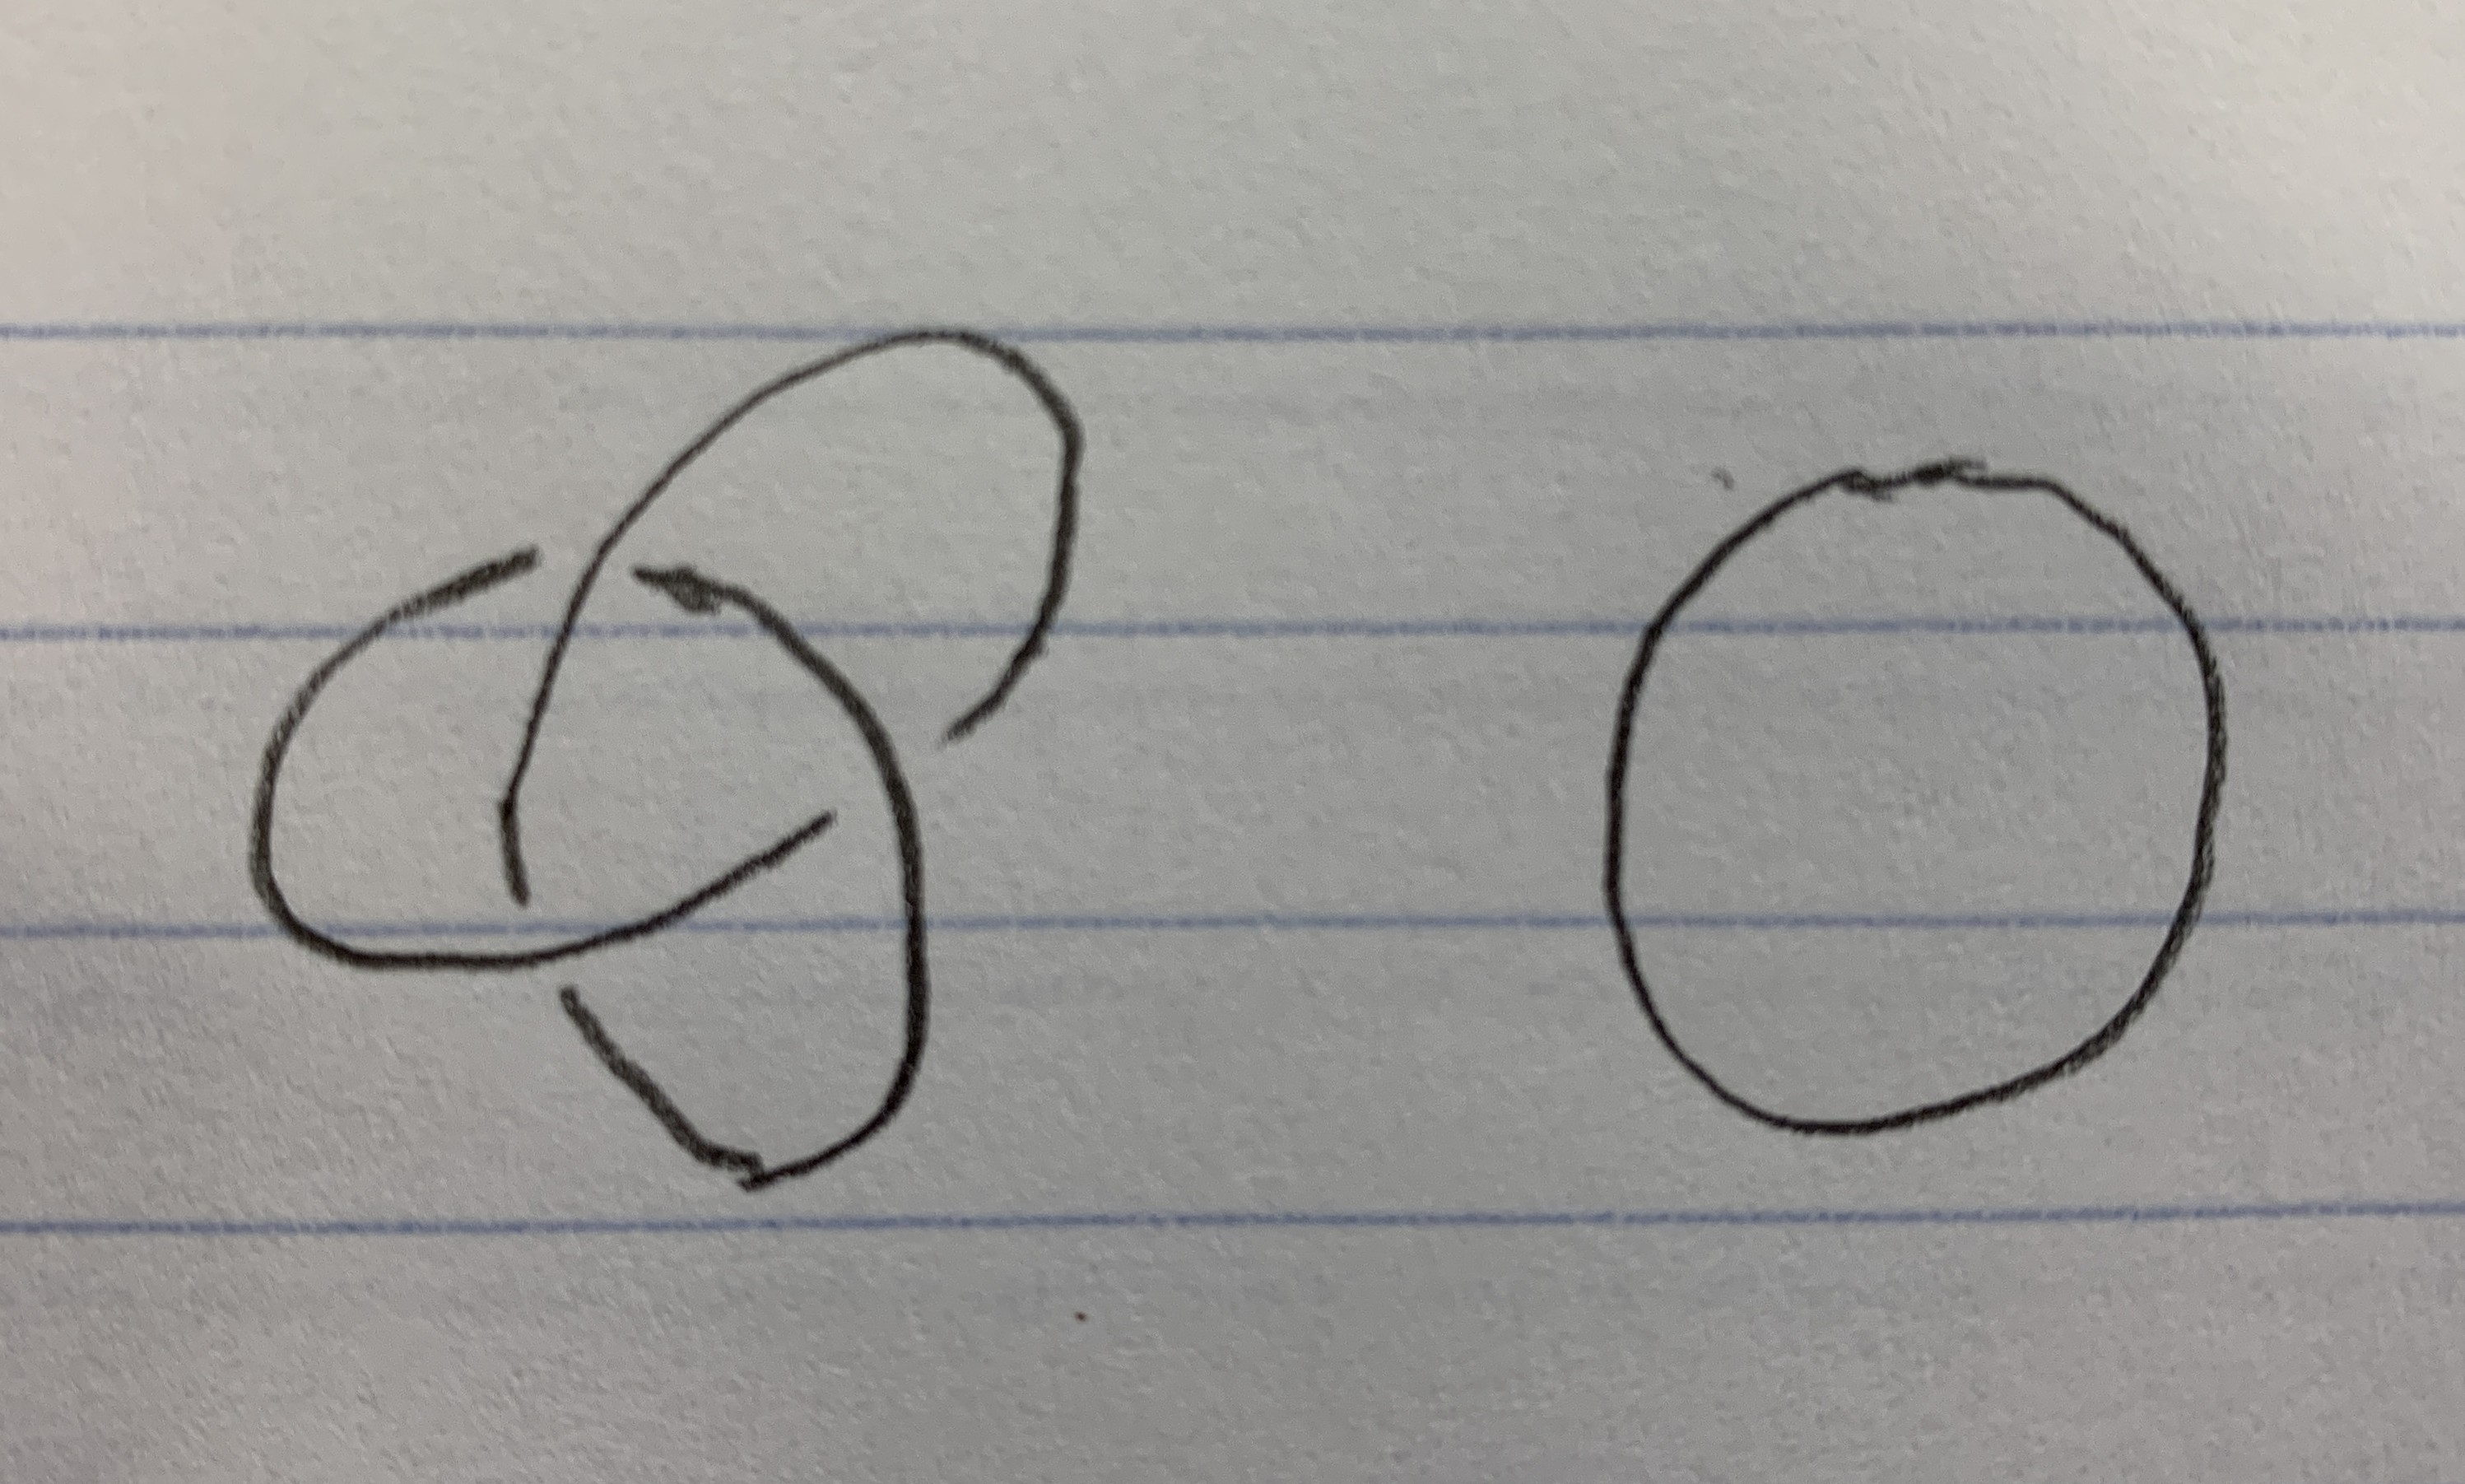
\includegraphics[width=0.7\textwidth]{img/knots.JPG}
        \end{center}

        \begin{itemize}
          \item
            A knot $K$ is equivalent to $K'$ if
            $(K, \mathbb{R}^3)$ is homeomorphic to $(K', \mathbb{R}^3)$

            In other words, there's a homeomorphism
            \[h : \mathbb{R}^3 \rightarrow \mathbb{R}^3 \text{ so that }
            h(K) = K'\]

            Then,
            \[h|_{\mathbb{R}^3-K} : \mathbb{R}^3-K \rightarrow \mathbb{R}^3-K'\]
            is also a homeomorphism,
        \end{itemize}
      \end{column}


      \begin{column}[T]{0.5\textwidth}
        \begin{itemize}
          \item
            ... and its induced homeomorphism from the fundemental groups
            \[\pi_1(\mathbb{R}^3-K) \rightarrow \pi_1(\mathbb{R}^3-K')\]
            is an isomorphism, so those groups are isomorphic.

          \item
            The group $\pi_1(\mathbb{R}^3) - K$ is also called the fundemental
            group of a knot.

          \item
            The main argument we'll be making is, if the fundemental groups of
            two knots aren't isomorphic, then the knots aren't equivalent.

          \item
            Seifert -- Van Kampen's Theorem helps determine the fundemental
            group of $A \cup B$ given the fundemental groups of $A$, $B$, and
            $A \cap B$.

          \item
            In this presentation, we'll be looking at the statement and proof
            of this theorem, and applying it to find the fundemental groups of a
            few knots.
        \end{itemize}
      \end{column}
    \end{columns}
  \end{frame}
  \begin{frame}
    \begin{columns}
      \begin{column}[T]{0.5\textwidth}
        \begin{itemize}
          \item The 'unknot' is the following knot:
          \item To say that a given knot can't be unknotted, we want to say
            that that knot is not equal to the unknot. So, before developing
            Seifert-Van Kampen's theorem, let's look at the fundemental group of
            the unknot:
          \item One nontrivial path is wrapping around the circle as shown.
            Similar to $\mathbb{R}^2-(0,0)$, it can be proved that any loops
            that wrap around the same number of times are equivalent (and loops
            that don't are not). So, the fundemental group is $<u>$.
        \end{itemize}
      \end{column}
    \end{columns}
  \end{frame}

  \begin{frame}
    \frametitle{Seifert -- Van Kampen Theorem}
    \begin{columns}
      \begin{column}[T]{0.5\textwidth}
        \begin{itemize}
          \item Let $X$ be a path-connected topological space, $x_0$ be any point
            in $X$. Let $\{U_\lambda\}_{\lambda \in \Lambda}$ be an open cover
            of $X$ so that each $U_\lambda$ contains $x_0$ and the intersection
            of any two elements in the cover is also in the cover.
          \item *here, $\{U_\lambda\}_{\lambda \in \Lambda}$ could be $\{A, B,
            A \cap B\}$*
          \item Let $\psi_\lambda$ be the homomorphism induced by the inclusion
                map $U_\lambda \rightarrow X$.
          \item
            \begin{minipage}[t]{0.5\textwidth}
              \vspace{-5.5mm}
              For $U_\lambda \subseteq U_\mu$, let $\phi_{\lambda\mu}$ be the
              homomorphism induced by the inclusion map $U_\lambda \rightarrow
              U_\mu$. Clearly, the following commutes:
            \end{minipage}%
            \begin{minipage}[t]{0.5\textwidth}
              \centering
              \vspace{-12mm}
                \[\begin{tikzcd}[ampersand replacement=\&]
                  \pi_1(U_\lambda) \ar[rd, "\psi_\lambda"]
                  \ar[r,"\phi_{\lambda\mu}"] \& \pi_1(U_\mu) \ar[d, "\psi_\mu"]
                  \\ \& \pi_1(X)
                  \end{tikzcd}\]
            \end{minipage}
          \item Let $H$ be any group and $\{p_\lambda\}_{\lambda \in \Lambda}$
            be any family of homomorphisms so the following commutes:
            \[\begin{tikzcd}[ampersand replacement=\&]
              \pi_1(U_\lambda) \ar[rd, "p_\lambda"]
              \ar[r,"\phi_{\lambda\mu}"] \& \pi_1(U_\mu) \ar[d, "p_\mu"]\\
                  \& H
              \end{tikzcd}\]
          \item Then, there's a unique $\sigma$ so that the following commutes:
            \[\begin{tikzcd}[ampersand replacement=\&]
                \pi_1(U_\lambda) \ar[rd, "p_\lambda"] \ar[r, "\psi_\lambda"] \&
                \pi_1(X) \ar[d, "\sigma"] \\
                  \& H
              \end{tikzcd}\]
        \end{itemize}
      \end{column}
      \begin{column}[T]{0.5\textwidth}
        From this definition, we can tell:
        \begin{itemize}
          \item If $\alpha \in \pi_1(U_\lambda)$, $\sigma(\psi_\lambda(\alpha)) = p_\lambda(\alpha)$
          \item If $\alpha \in \pi_1(U_\lambda)$, $\beta \in \pi_1(U_\mu)$,
            \[\sigma(\psi_\lambda(\alpha)\psi_\mu(\beta)) =
            \sigma(\psi_\lambda(\alpha))\sigma(\psi_\mu(\beta)) =
            p_\lambda(\alpha)p_\mu(\beta)\]
          \item For $\{\alpha_i\}_{i=1}^n$ so that $\alpha_i \in U_{\lambda_i}$,
            \[\sigma(\psi_{\lambda_1}(\alpha_1)\psi_{\lambda_2}(\alpha_1) ...
            \psi_{\lambda_n}(\alpha_n)) = p_{\lambda_1}(\alpha_1)p_{\lambda_2}(
            \alpha_2) ... p_{\lambda_n}(\alpha_n)\]
          \item We need to prove that $\sigma$ is well defined, In other words,
            if
            \[\psi_{\lambda_1}(\alpha_1) \psi_{\lambda_2}(\alpha_2) ...
              \psi_{\lambda_n}(\alpha_n) \sim \psi_{\mu_1}(\beta_1)
              \psi_{\mu_2}(\beta_2) ... \psi_{\mu_m}(\beta_m)\]
            Then, $\sigma(\psi_{\lambda_1}(\alpha_1) ...
              \psi_{\lambda_n}(\alpha_n)) \sim \sigma(\psi_{\mu_1}(\beta_1) ...
              \psi_{\mu_m}(\beta_m))$
 
            So, \quad \quad \ \ $p_{\lambda_1}(\alpha_1) ... p_{\lambda_n}(\alpha_n)
              \sim p_{\mu_1}(\beta_1) ... p_{\mu_m}(\beta_m)$
          \item Since this is all the restrictions on $\sigma$, but $\sigma$ is
            unique, $\pi_1(X)$ must not have any elements which aren't in the
            form
              \[\psi_{\lambda_1}(\alpha_1) \psi_{\lambda_2}(\alpha_2) ...
              \psi_{\lambda_n}(\alpha_n)\]
            We also need to prove this.
          \item We'll also look at when two elements of $\pi_1(X)$ are equal and
            when they're different.
          \item But hopefully it makes sense how this theorem determines
            $\pi_1(X)$!
        \end{itemize}
      \end{column}
    \end{columns}
  \end{frame}
  \begin{frame}
    \frametitle{Seifert -- Van Kampen Theorem Proof -- Part 1}
    \begin{columns}
      \begin{column}[T]{0.5\textwidth}
        \begin{itemize}
          \item To Prove: Every element of $a$ $\pi_1(X)$ can be expressed as
            \[a = \psi_{\lambda_1}(\alpha_1)\psi_{\lambda_2}(\alpha_2) ...
              \psi_{\lambda_n}(\alpha_n)\]
            for $\lambda_i \in \Lambda, \alpha_i \in U_{\lambda_i}$.
          \item We will use:

            Lebesgue's Number Lemma: Every open cover of a compact metric space
            has a $\delta$ so that any subset of the metric space with diameter
            less than $\delta$ is contained in a single element of the cover.
            $\delta$ is called the Lebesgue number of the cover.
          \item For any $a \in \pi_1(X)$, find a path $f : [0,1] \rightarrow X$
            so that $a = [f]_{\pi_1(X)}$.
          \item $\{f^{-1}(U_\lambda)\}_{\lambda
            \in \Lambda}$ is a cover of the compact metric space $[0,1]$. It
            has a Lebesgue number $\delta$.
          \item Find $n$ so $\frac{1}{n} < \delta$, divide $[0,1]$ into
            subintervals $[0,\frac{1}{n}]$, $[\frac{1}{n}, \frac{2}{n}]$, ...,
            $[\frac{n-1}{n},1]$. Each has diameter less than $\delta$, so
            $[\frac{i}{n}, \frac{i+1}{n}] \in f^{-1}(U_{\lambda_i})$ for some
            $\lambda_i$, and $f([\frac{i}{n}, \frac{i+1}{n}]) \in U_{\lambda_i}$.
          \item Let $f_i$ be $f$ from $f(\frac{i-1}{n})$ to $f(\frac{i}{n})$. So,
              \[f \sim f_1 f_2 f_3 ... f_n\]
          \item $f(\frac{i}{n}) \in U_{\lambda_i}, U_{\lambda{i+1}}$. Since
            $U_{\lambda_i} \cap U_{\lambda_{i+1}} \in \{U_\lambda\}_{\lambda
            \in \Lambda}$, and all elements of $\{U_\lambda\}_{\lambda \in
            \Lambda}$ are path connected and include $x_0$, there's a path $k_i$
            from $f(\frac{i}{n})$ to $x_0$ contained in $U_{\lambda_i} \cap
            U_{\lambda_{i+1}}$.

        \end{itemize}
      \end{column}
      \begin{column}[T]{0.5\textwidth}

        \begin{center}
          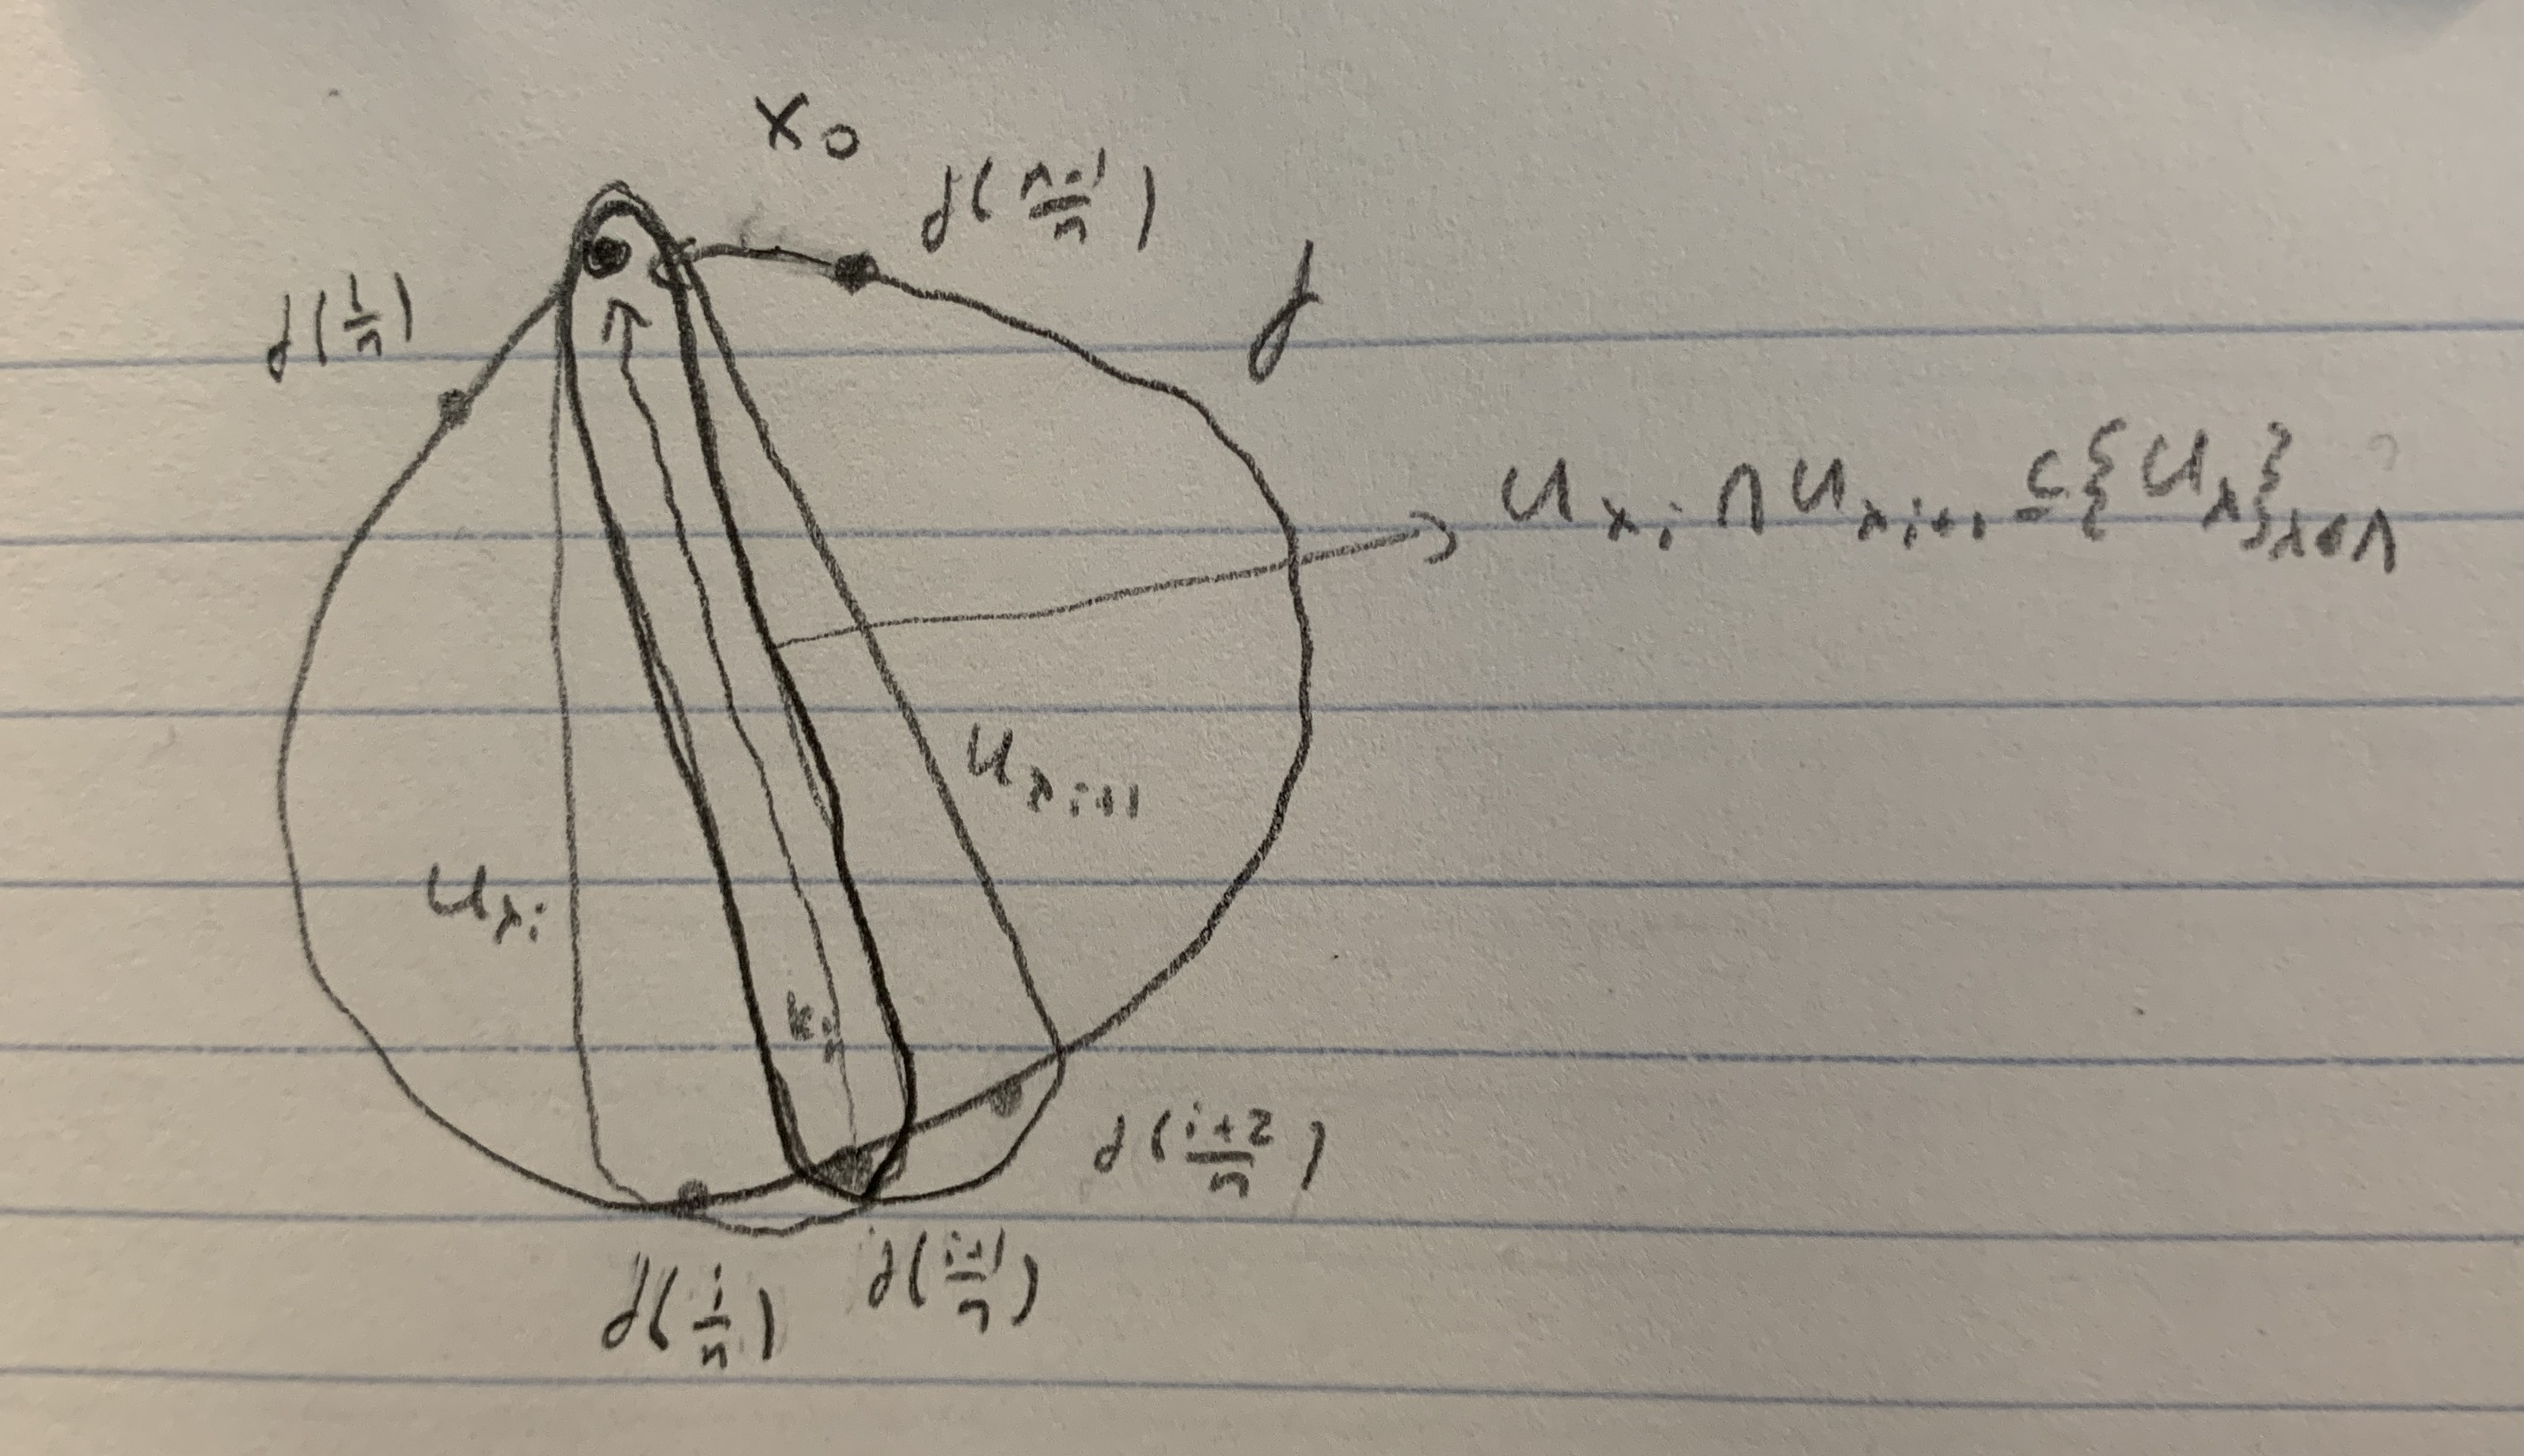
\includegraphics[width=0.7\textwidth]{img/proof-pt1.JPG}
        \end{center}
        \begin{itemize}
          \item We add the $k_i$ to put each small piece starts and ends at $x_0$,
            and so is in a fundemental group:
              \[f \sim f_1k_1\cdot k_1^{-1}f_2k_2 \cdot k_2^{-1}f_3k_3 \cdot ... \cdot k_{n-1}^{-1}f_n\]
              \[a = [f]_{\pi_1(X)} = [f_1k_1]_{\pi_1(X)} [k_1^{-1}f_2k_2]_{\pi_1(X)}
                 ... [k_{n-1}^{-1}f_n]_{\pi_1(X)}\]
            Now, $k_{i-1}f_ik_i \subseteq U_{\lambda_i}$, since $k_i \subseteq
            U_{\lambda_i}, U_{\lambda_{i+1}}$. Since $\psi_{\lambda_i}$ is the
            homomorphism induced by an inclusion map,
              \[ a = \psi_{\lambda_1}([f_1k_1]_{\pi_1(U_{\lambda_1})}) ...
                \psi_{\lambda_n}( [k_{n-1}f_n]_{\pi_1(U_{\lambda_n})})\]

        \end{itemize}
      \end{column}
    \end{columns}
  \end{frame}
  \begin{frame}
    \frametitle{Seifert -- Van Kampen Theorem Proof -- Part 2}
    \begin{columns}
      \begin{column}[T]{0.5\textwidth}
        \begin{itemize}
          \item We'd like to show that
              \[\psi_{\lambda_1}(\alpha_1) ... \psi_{\lambda_n}
            (\alpha_n) = \psi_{\mu_1}(\beta_1) ... \psi_{\mu_m}(\beta_m)\]
            Implies
             \[p_{\lambda_1}(\alpha_1) ... p_{\lambda_n}(\alpha_n) =
              p_{\mu_1}(\beta_1) ... p_{\mu_1}(\beta_1) \]

            Since paths are invertible, and everything involved is a homomorphism,
            we can put everything on one side:

            \[\psi_{\lambda_1}(\alpha_1) ... \psi_{\lambda_n}(\alpha_n)
              \psi_{\mu_m}(\beta_m^{-1}) ... \psi_{\mu_1}(\beta_1^{-1}) = 1\]

            Implies
              \[p_{\lambda_1}(\alpha_1) ... p_{\lambda_n}(\alpha_n)
              p_{\mu_m}(\beta_m^{-1}) ... p_{\mu_1}(\beta_1^{-1}) = 1\]

            So, it'll suffice to show,
            $\psi_{\lambda_1}(\alpha_1) ... \psi_{\lambda_n}(\alpha_n) = 1$ implies
            $p_{\lambda_1}(\alpha_1) ... p_{\lambda_n}(\alpha_n) = 1$

            Let $f_i$ represent $\psi_{\lambda_i}(\alpha_i)$ so
            $\psi_{\lambda_i}(\alpha_i) = [f_i]_{\pi_1(X)}$.
            If $\psi_{\lambda_1}(\alpha_1) ... \psi_{\lambda_n}(\alpha_n) = 1$,
            there's a continuous function $F : [0,1]x[0,1] \rightarrow X$ with
            $F(1,t) = F(s,0) = F(s,1) = x_0$,
            \[F(0,t) = \begin{cases} f_1 & [0,\frac{1}{n}) \\ f_2 & [\frac{1}{n}, \frac{2}{n}) \\ ... \end{cases}\]

        \end{itemize}
      \end{column}
      \begin{column}[T]{0.5\textwidth}
        \begin{itemize}
          \item Using the Lebesgue number, split up $[0,1]x[0,1]$ into rectangles
            so each fits in a single $U_\lambda$, making sure that each $\frac{i}{n}$ is at a boundary:
            \begin{center}
              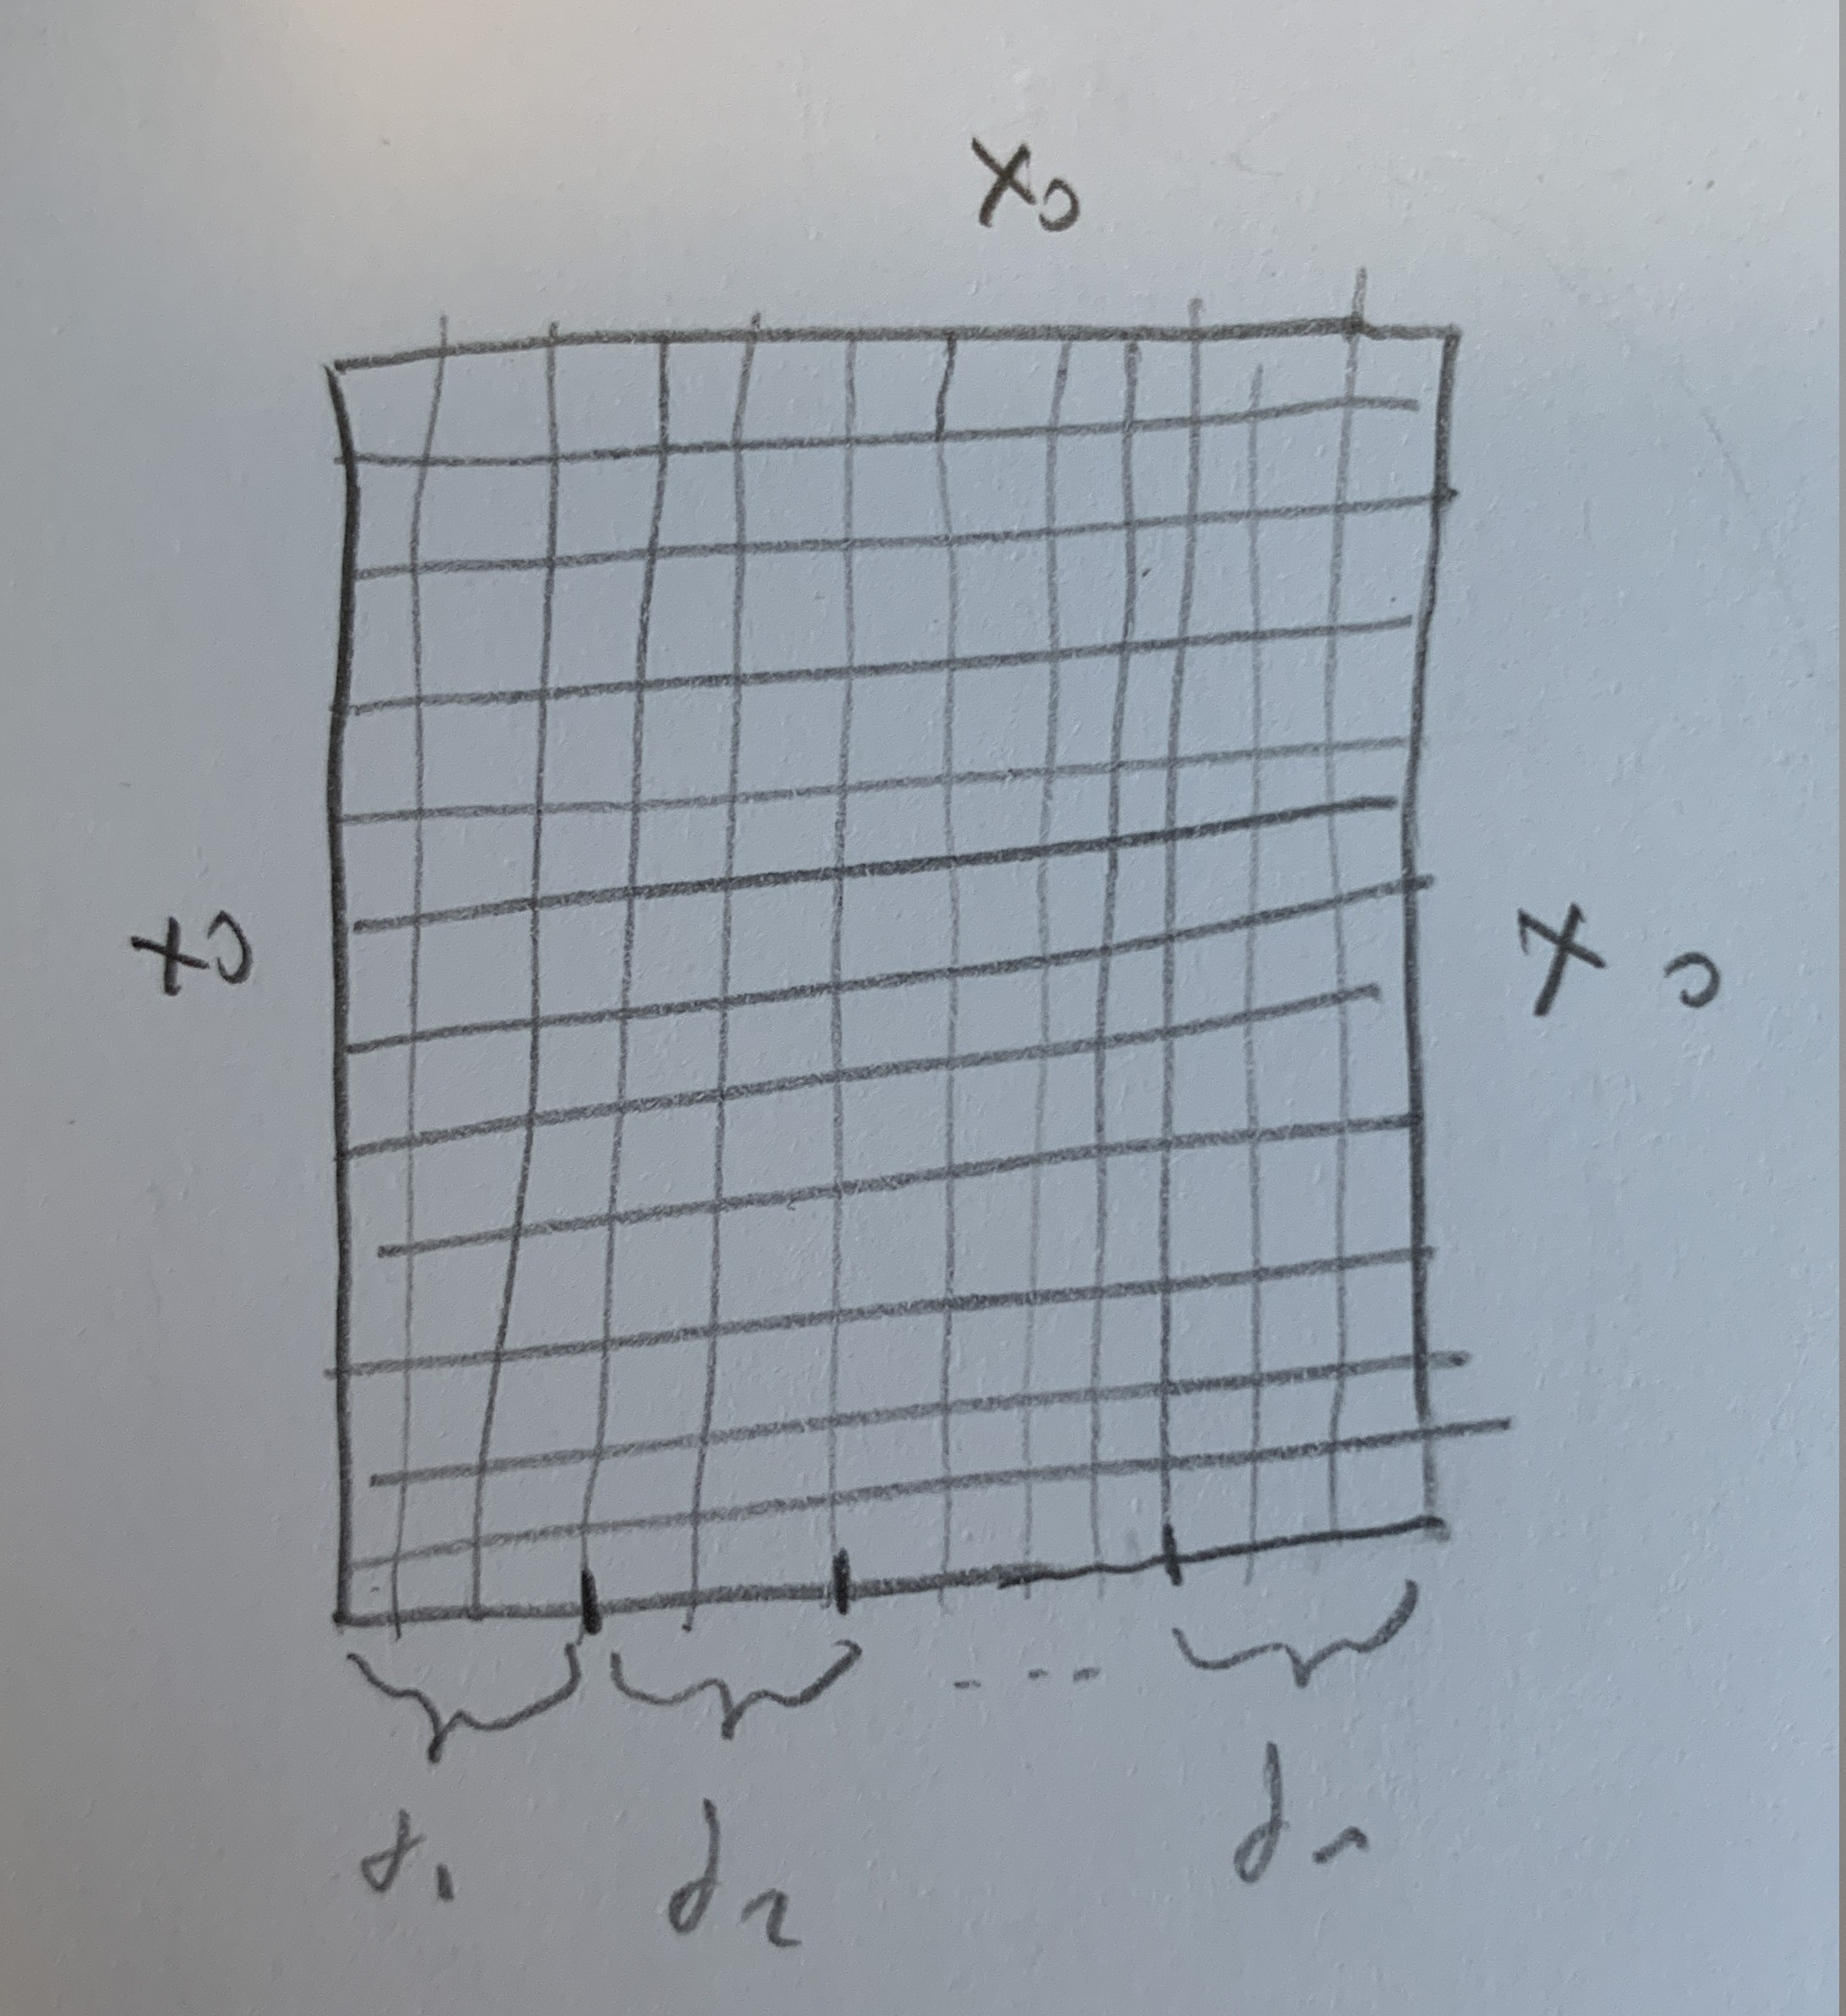
\includegraphics[width=0.4\textwidth]{img/proof-pt2-overview.JPG}
            \end{center}
          \item For each intersection, add a line $k_{ij}$ going from the intersection to $x_0$, contained in the $U_\lambda$'s of all four surrounding rectangles.
          \item In each line below, add $k_{ij}$'s as necessary to put them in the fundemental group:

            For each rectangle, since it's contained in $U_\lambda$,
            \begin{center}
              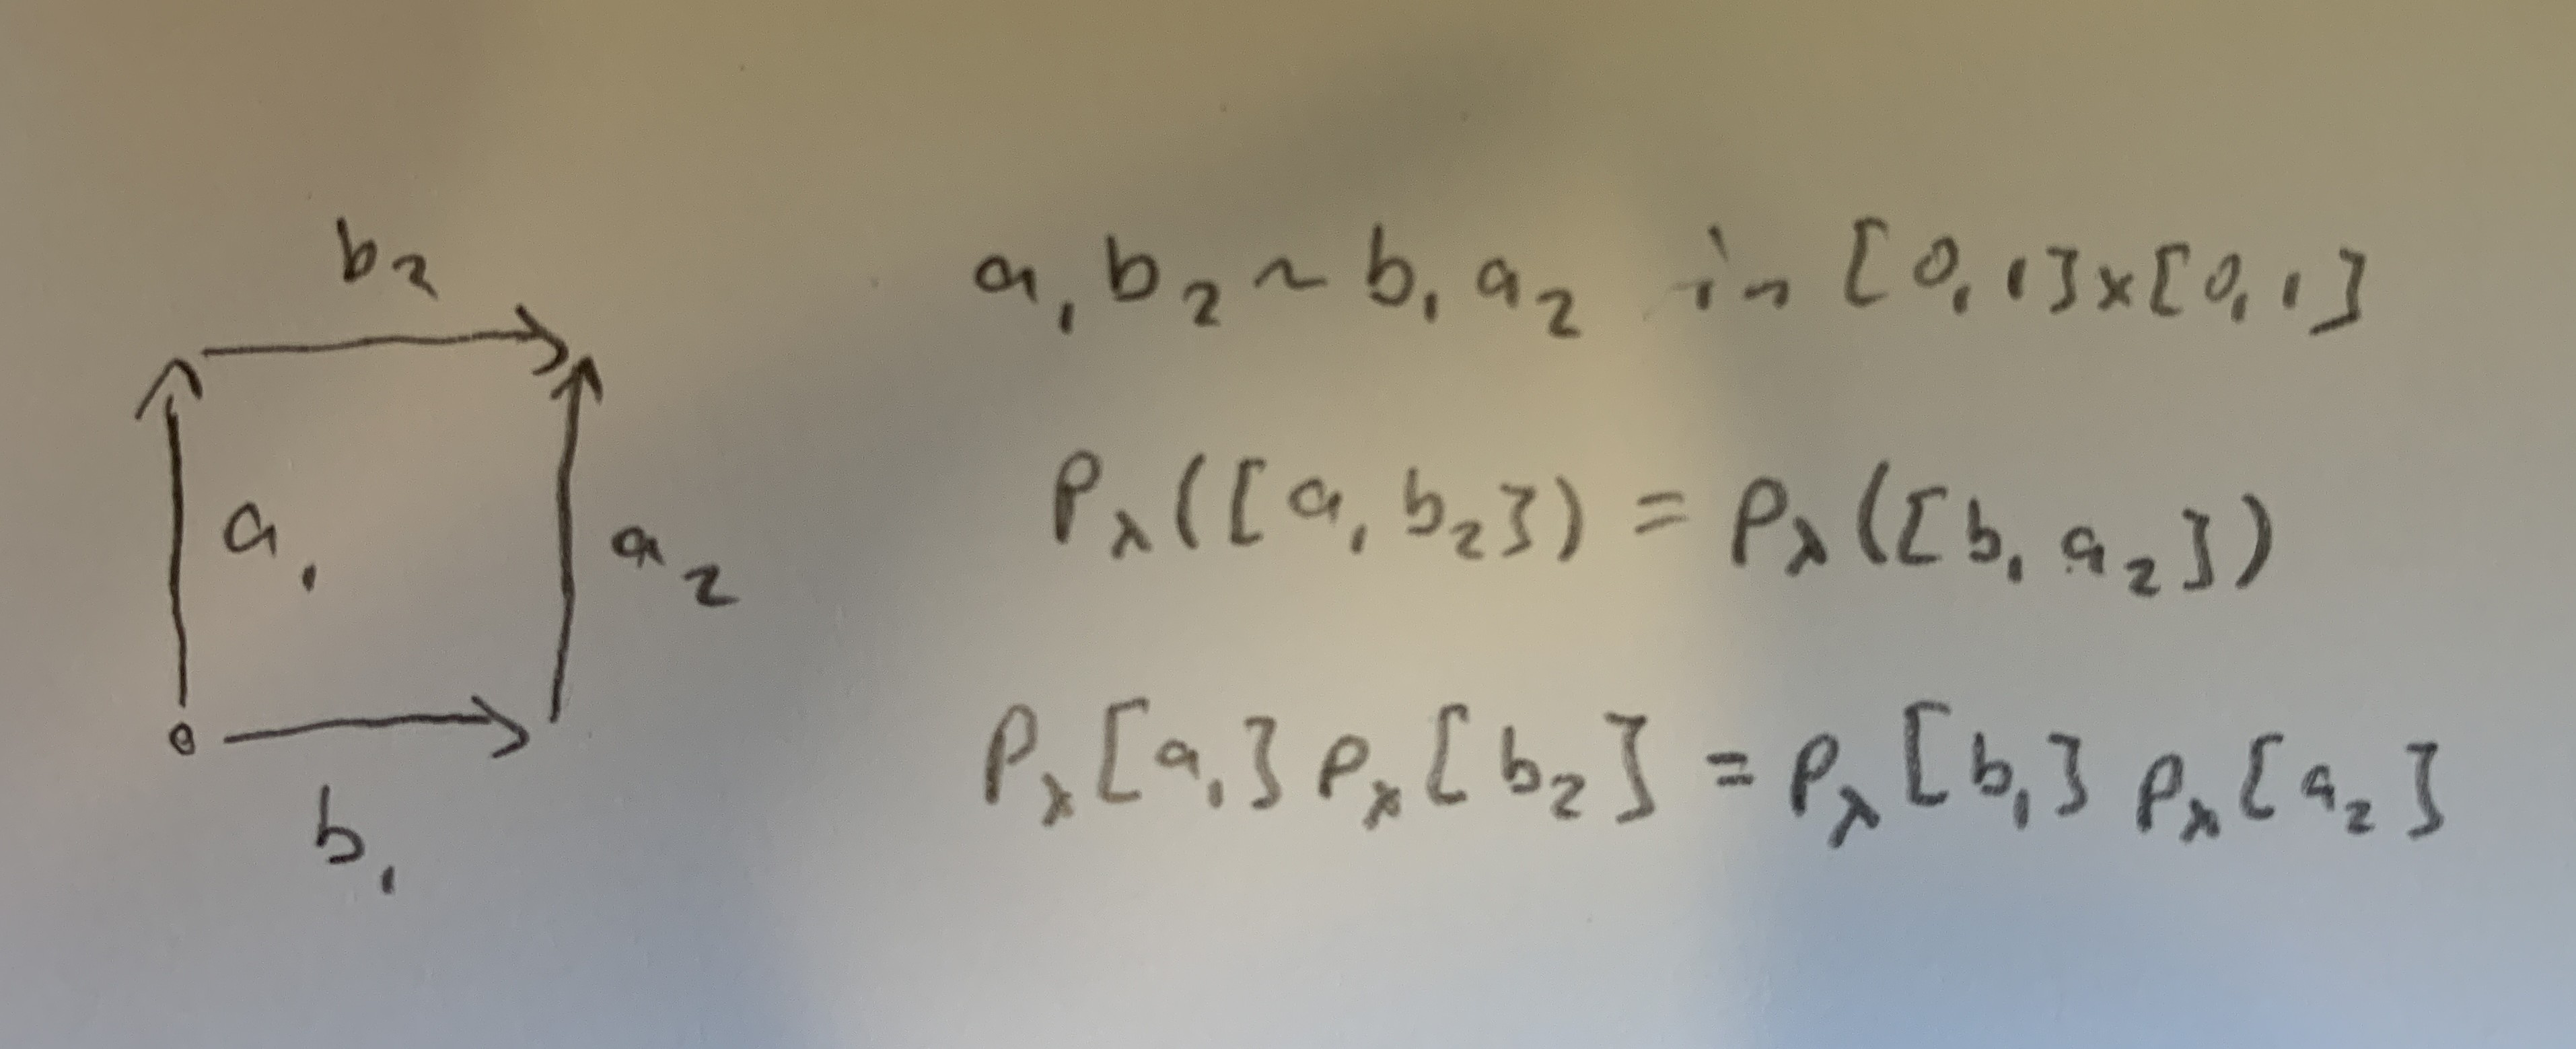
\includegraphics[width=0.7\textwidth]{img/proof-pt2-each-rectangle.JPG}
            \end{center}

          \end{itemize}
      \end{column}
    \end{columns}
  \end{frame}
  \begin{frame}
    \begin{columns}
      \begin{column}[T]{0.5\textwidth}
        \begin{itemize}
          \item Now, remember that
            \[\begin{tikzcd}[ampersand replacement=\&]
              \pi_1(U_\lambda) \ar[rd, "p_\lambda"]
              \ar[r,"\phi_{\lambda\mu}"] \& \pi_1(U_\mu) \ar[d, "p_\mu"]\\
                  \& H
              \end{tikzcd}\]
            \begin{center}
              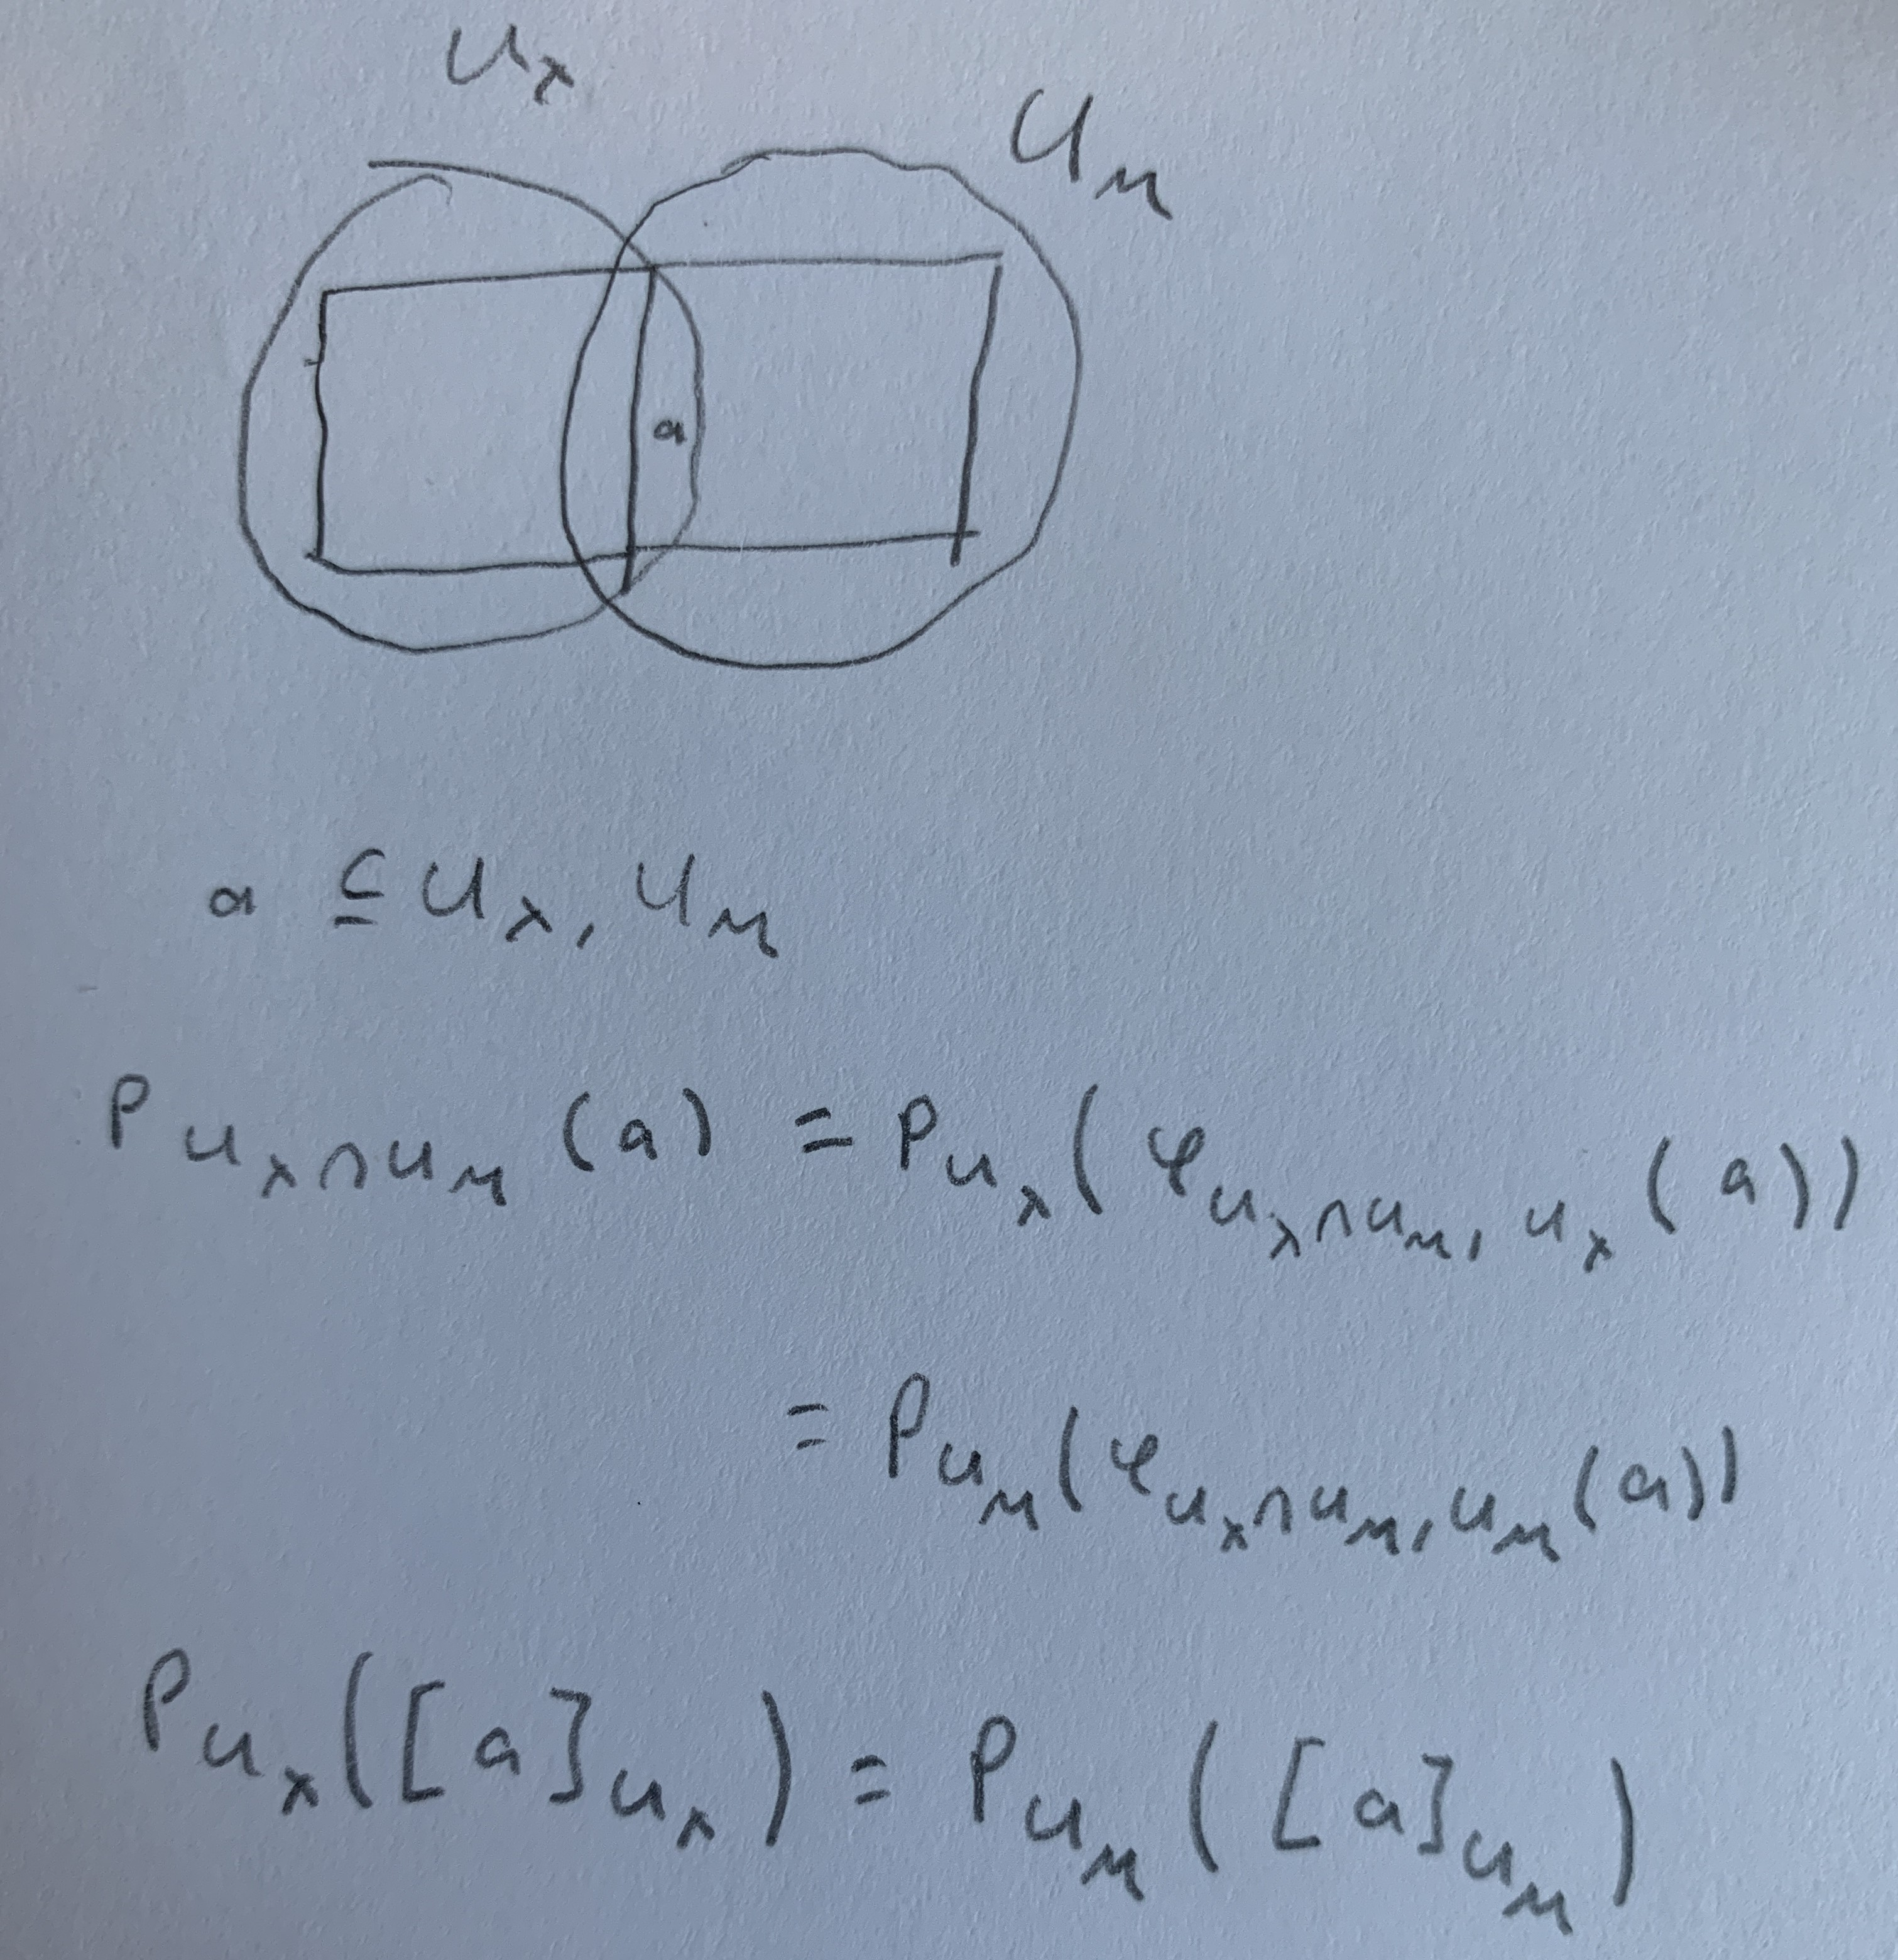
\includegraphics[width=0.5\textwidth]{img/proof-pt2-pair-rectangle.JPG}
            \end{center}

          \item Notice that along the left, top, and right edges, $p$ of the trivial
            loops is $1$, so the whole composition is $1$.

          \item Now, we can apply the previous two parts a finite number of times to
            move that composition to the bottom without changing its value:


        \end{itemize}
      \end{column}
      \begin{column}[T]{0.5\textwidth}
            \begin{center}
              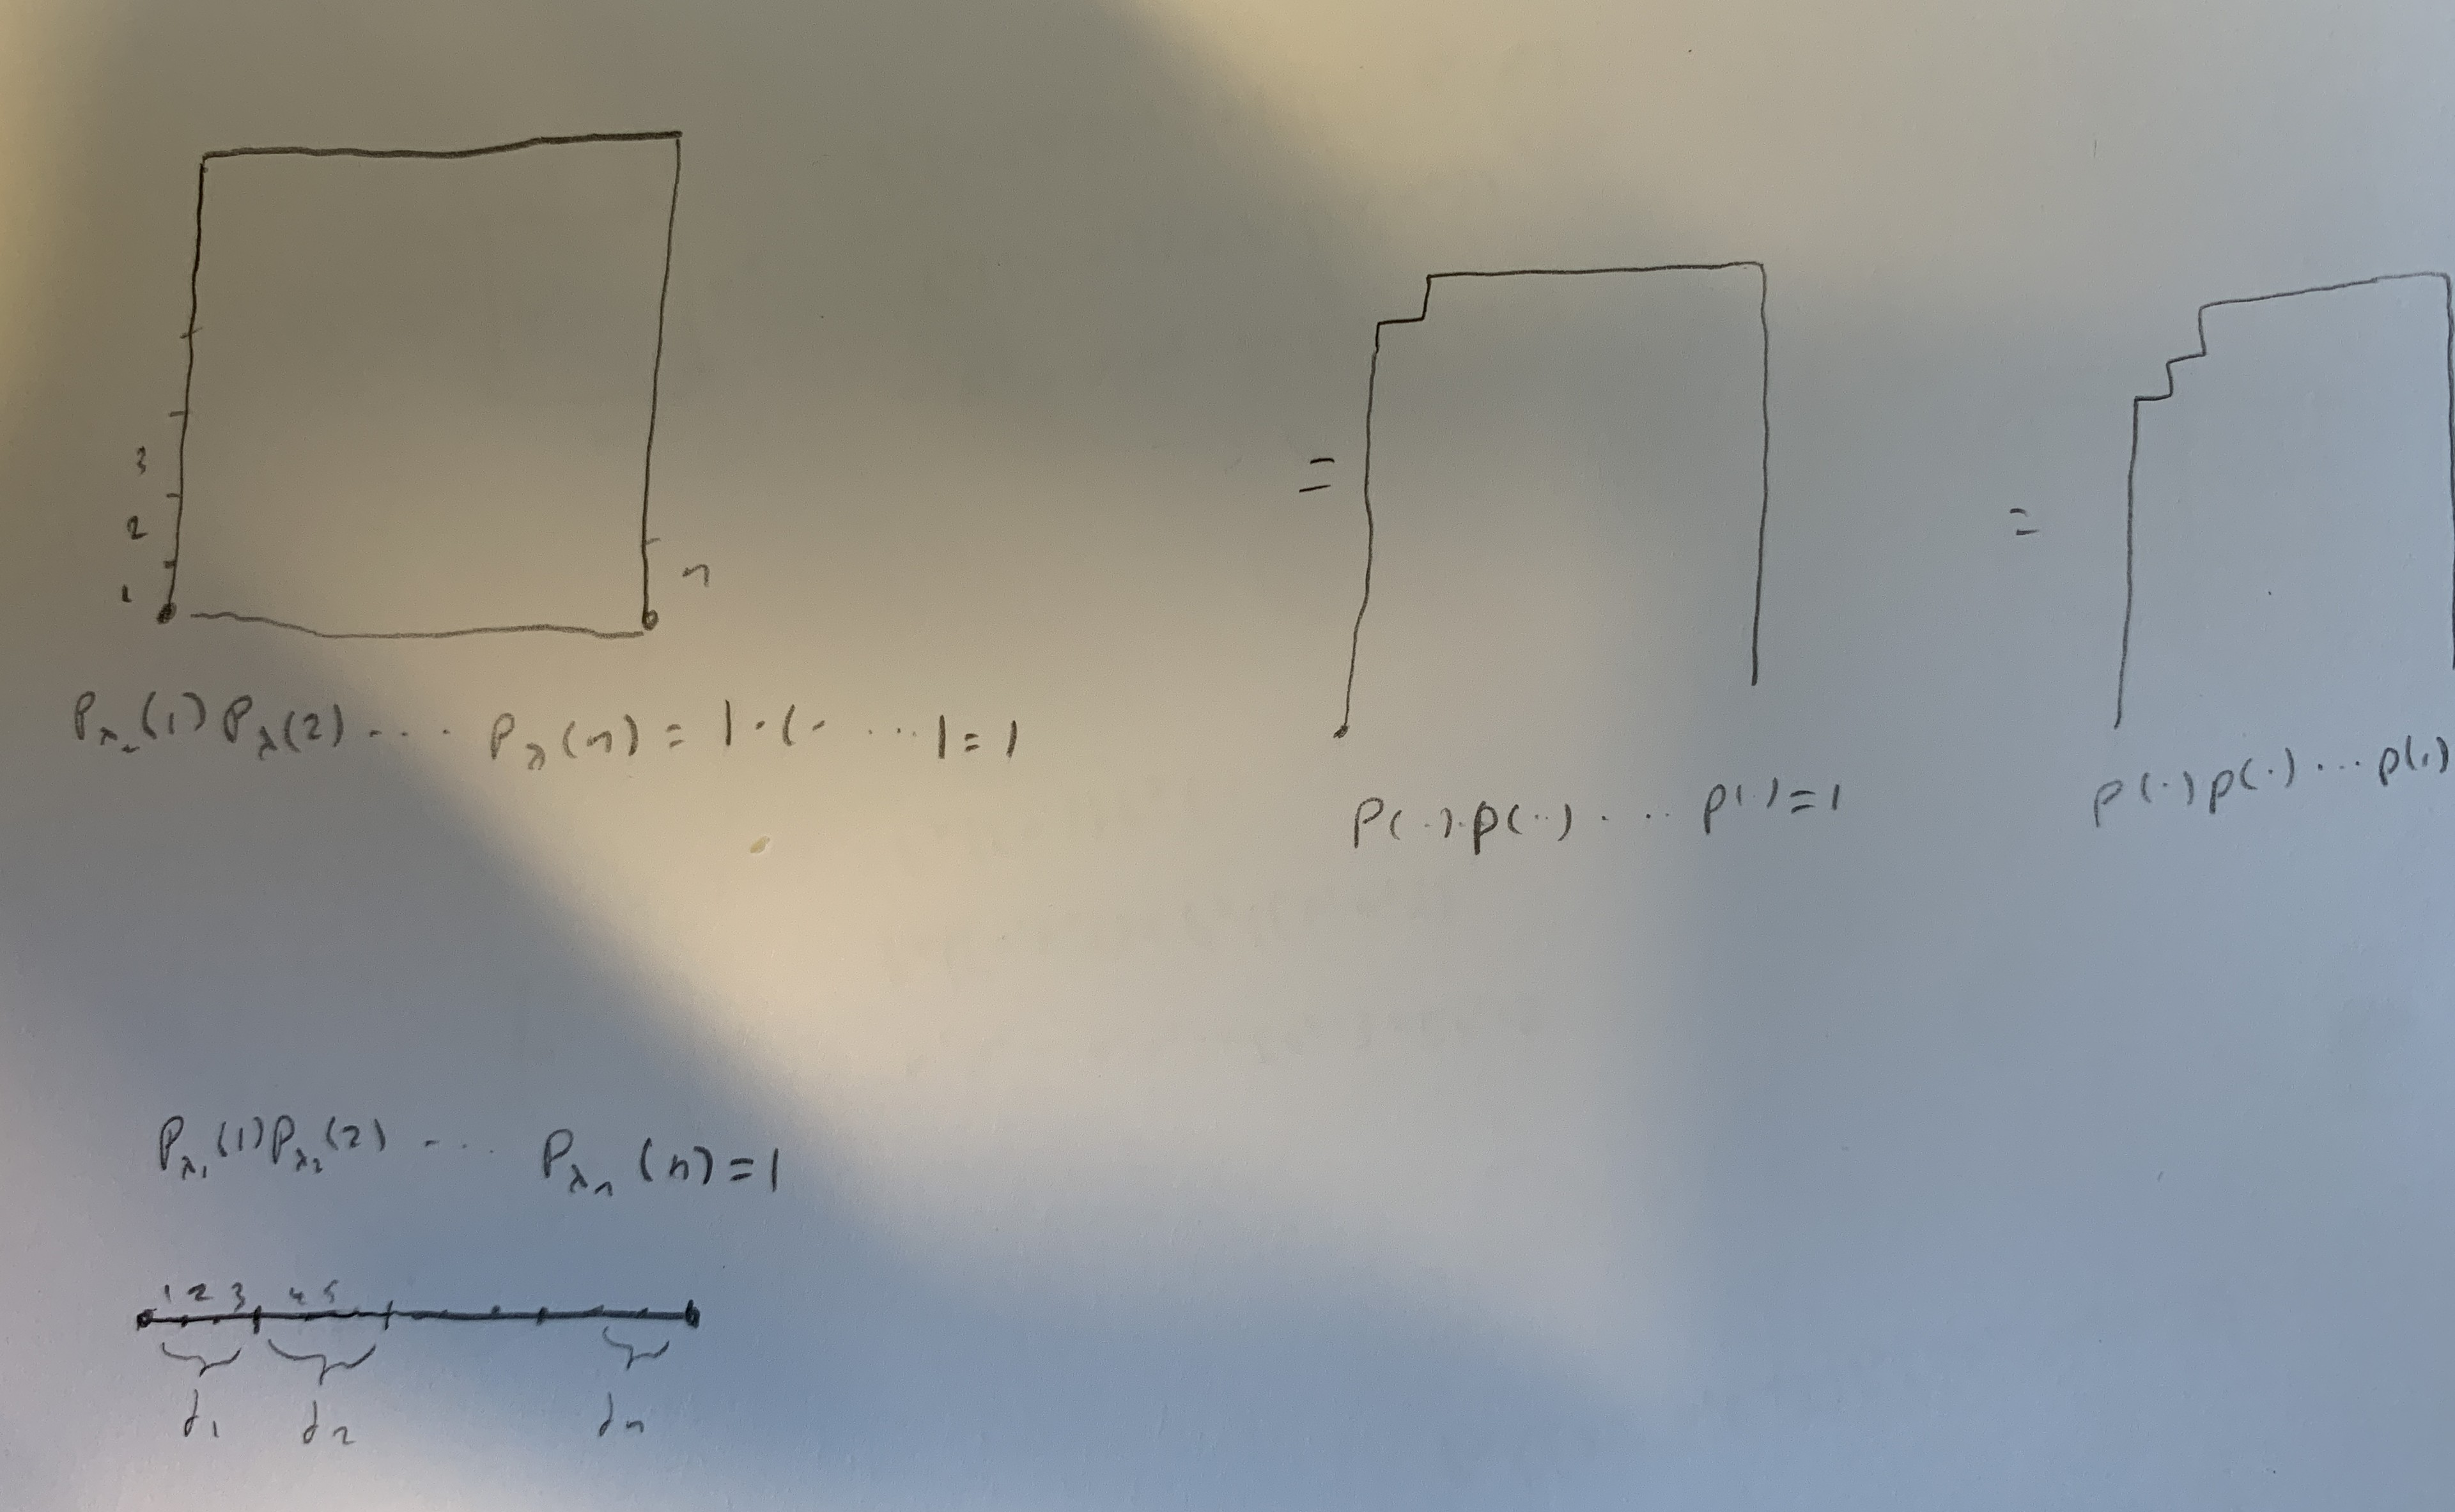
\includegraphics[width=0.7\textwidth]{img/proof-pt2-ending.JPG}
            \end{center}
        \begin{itemize}
          \item
            Finally, since each $f_i$ is contained in a $U_{\mu_i}$,
            \[\underbrace{p_{\lambda_1}([1]_{U_{\lambda_1}})p_{\lambda_2}([2]_{U_{\lambda_2}})p_{\lambda_3}([3]_{U_{\lambda_3}})}_{f_1} \underbrace{p_{\lambda_4}([4]_{U_{\lambda_4}})p_{\lambda_5}([5]_{U_{\lambda_5}})}_{f_2} ... = 1\]
            \[\underbrace{p_{\mu_1}([1]_{U_{\mu_1}})p_{\mu_1}([2]_{U_{\mu_1}})p_{\mu_1}([3]_{U_{\mu_1}})}_{f_1} \underbrace{p_{\mu_2}([4]_{U_{\mu_2}})p_{\mu_2}([5]_{U_{\mu_2}})}_{f_2} ... = 1\]
            \[\underbrace{p_{\mu_1}([123]_{U_{\mu_1}})}_{f_1} \underbrace{p_{\mu_2}([45]_{U_{\mu_2}})}_{f_2} ... = 1\]
          \item Since we know $F$ maps those sections to $f_i$,

            \[p_{\mu_1}([f_1])p_{\mu_2}([f_2]) ... p_{\mu_n}([f_n]) = 1\]
        \end{itemize}
      \end{column}
    \end{columns}
  \end{frame}
  \begin{frame}
    \frametitle{Seifert -- Van Kampen Theorem, corollary}

    \begin{columns}
      \begin{column}[T]{0.5\textwidth}
        \begin{itemize}
          \item We will prove: If $X = U \cup V$, $\pi(X) = \frac{\pi(U) * \pi(V)}{N}$ where $N$ is the smallest subgroup containing $\phi_{U \cap V, U}(x)\phi_{U \cap V, V}(x)^{-1}$ for all $x$ in $U \cap V$.
          \item Elements of the free product $\pi(U) * \pi(V)$ are strings like $u_1v_1u_2..v_n$, where each $u_i$ is in $\pi(U)$ and each $v_i$ is in $\pi(V)$. If two adjacent elements are in the same group, you can apply that group's operation:
            \[u_1u_2v_1 = (u_1 \cdot_{\pi_U}u_2)v_3\]
            
            In terms of generators and relations, if $\pi(U) = <u_1, u_2, ...: r_1, r_2, ...>$, $\pi(V) = <v_1, v_2, ...: r'_1, r'_2, ...>$, and $\pi(U \cap V) = <w_1, w_2, ...: r''_1, r''_2, ...>$, then
          \[\pi(U)*\pi(V) = <u_1, u_2, ..., v_1, v_2, ... : r_1, r_2, ..., r
            r'_1, r'_2, ...>\]
          \[\frac{\pi(U) * \pi(V)}{N} = <u_1, u_2, ..., v_1, v_2, ... : r_1, r_2, ..., r
            r'_1, r'_2, ..., i_U(w_1)i_V(w_1)^{-1}, i_U(w_2)i_V(w_2)^{-1}, ...>\]

          \item Proof: We can define a function $F : \pi(U) * \pi(V) \rightarrow \pi(X)$, by
            \[F(u_1v_1u_2...v_n) = \psi_U(u_1)\psi_V(v_1)\psi_U(u_2) ... \psi_V(v_n)\]
            If $i_U(x)i_V(x)^{-1} \in N$,
            \[F(i_U(x)i_V(x)^{-1}) = \psi_U(i_U(x))\psi_V(i_V(x))^{-1} = 1\]
            So, $N$ is in the kernel of $F$ and the function $F$ is well defined $\frac{\pi(U)*\pi(V)}{N} \rightarrow \pi(X)$.
            By the proof of Seifert - Van Kampen's theorem, part 1, we know that
            elements $\psi_U(u_1)\psi_V(v_1)\psi_U(u_2) ... \psi_V(v_n)$ generate
            $\pi(X)$, $F$ is surjective onto $\pi(X)$.
            We also have:
            \[i_1: \pi(U) \rightarrow \frac{\pi(U)*\pi(V)}{N}, i_1(u) = u\]
            \[i_2: \pi(V) \rightarrow \frac{\pi(U)*\pi(V)}{N}, i_1(v) = v\]
            \[i_3: \pi(U \cap V) \rightarrow \frac{\pi(U)*\pi(V)}{N}, i_1(x) = i_U(x) = i_V(x)\]
            where the last two elements are equal in the quotient group since $i_U(x)i_V(x)^{-1} \in N$.

            Then, we can apply Seifert - Van Kampen's theorem and get $\sigma : \pi(X) \rightarrow \frac{\pi(U)*\pi(V)}{N}$.
            The following commutes:
            \[\begin{tikzcd}[ampersand replacement=\&]
                \pi_1(U) \ar[rd, "i_1"] \ar[r, "i_U"] \&
                \pi_1(X) \ar[d, "\sigma"] \\ \& H \end{tikzcd}\]
            So, if $u \in \pi(U)$, $(\sigma \cdot F)(u) = \sigma(i_U(u))=i_1(u)
            = u$. Similarly, $(\sigma \cdot F)(v) = v$ for $v \in \pi(V)$.

            Since elements of $\pi(U)$ and $\pi(V)$ generate $\pi(U)*\pi(V)$,
            which generates $\frac{\pi(U)*\pi(V)}{N}$. So, this means $\sigma
            \cdot F$ is the identity function, so $F$ is injective. Therefore,
            $F$ is an isomorphism and the groups $\pi(X)$ and $\frac{\pi(U)*
            \pi(V)}{N}$ are isomorphic.
        \end{itemize}
      \end{column}
    \end{columns}
  \end{frame}
            
  \begin{frame}
    Calculating the group of the trefoil knot
    \begin{columns}
      \begin{column}[T]{0.5\textwidth}
        \begin{itemize}
          \item Let's consider the following knot:
            %image
          \item We can draw a torus that includes this knot:
            %image
          \item Then, split the space $R^3 - K$ into three sections:
          
            $U$: inside the torus, including the boundary (but not $K$)

            $V$: outside the torus, including the boundary (but not $K$)

            $U \cap V$: the boundary of the torus, not including $K$.

          \item The fundemental group of $U$ is essentially the same as the fundemental
          group of $S^1$, which is $<u>$, where $u$ is a loop going aroung the hole

          \item The fundemental group of $V$ is essentially the same as the fundemental group
            of $R^3 - S^1$, which we saw is $<v>$ where $v$ is the loop in the picture:

          \item $U \cap V$ is essentially just a strip in $R^3$, so its
            fundemental group is going around once in the strip, $<w>$.

          \item $w$ goes around the torus two times, so $i_U(w) = u^2$. It rotates three times,
            around the outside, so $i_V(w) = v^3$.

          \item By Seifert -- Van Kampen's theorem, $\pi(R^3 - K) = <u,v,u^2 = v^3>$
        \end{itemize}
      \end{column}
    \end{columns}
  \end{frame}
  \begin{frame}
    \frametitle{Wirtinger Presentation}
    \begin{columns}
      \begin{column}[T]{0.5\textwidth}
        \begin{itemize}
          \item Take any 'drawing' of a knot as curves and put it in
            $\mathbb{R}^3$ as shown. Draw lines $a_i$ going across every section
            of the knot.
          \item At every intersection, there are one of two intersections $r_i$.
          \item Divide up $\mathbb{R}^3$ as follows:
          \item $A = \{(x,y,z): z >= -1\}$. In $A$, each line segments forms a
            handle, and the fundemental group of $A$ is going through any number
            of them in any order, so $<a_1, ... a_n>$.
          \item $B_i$: rectangular box under every intersection, with its top at
            $z = -1$. Any path in the rectangular box is trivial, so its fundemental group is $1$.
          \item $C$: Anything below $A$ and all the $B$'s. Its fundemental group is $1$ as well.

            We'll take $A$ and add the $B_i$'s one by one. $A \cap B_1$ is a
            rectangle with a line segment in the middle cut out. So, its
            fundemental group is generated by going around that line segment
            once, which, included in $A$ is exactly $r_i$. So, the fundemental
            group is $<a_1, ... a_n : r_1>$.

            Adding the other $B_i$'s one by one, the fundemental group becomes
            \[<a_1, a_2, ... a_n : r_1, r_2, ... r_n>\]
            The intersection of $A \cup B_1 ... \cup B_n$ and $C$ also has a
            trivial fundemental group so the fundemental group of the union of
            all the parts, $\mathbb{R}^3- K$ is
            \[\pi(\mathbb{R}^3-K) = <a_1, a_2, ... a_n : r_1, r_2, ... r_n>\]

        \end{itemize}
      \end{column}
    \end{columns}
  \end{frame}
  \begin{frame}
    \frametitle{Do we get the same group with the Wirtinger Presentation?}
    \begin{columns}
      \begin{column}[T]{0.5\textwidth}
        \begin{itemize}
          \item For the trefoil, we get three line segments and three relations
            as shown.
            \[\pi(\mathbb{R}^3-K) = <a_1, a_2, a_3: a_1a_3 = a_2a_1, a_2a_1 = a_3a_2, a_3a_2 = a_2a_1>\]
            Clearly, the first two relations imply the third, so this group is equivalent to
            \[<a_1, a_2, a_3: a_1a_3 = a_2a_1, a_2a_1 = a_3a_2>\]
            We can solve the first relation for $a_3$ to get $a_3 =
            a_1^{-1}a_2a_1$. So, any string of $a_1$,$a_2$, $a_3$ is also
            generated by $a_2$ and $a_3$ with $a_1$ as this expression. So, we
            get:
            \[<a_2, a_3: , a_2a_1 = a_1^{-1}a_2a_1a_2>\]
            \[<u, v: , uvu = vuv>\]
            \[uvu*uvu = vu*vu*vu\]
            Let $w = uvu$, $z = vu$. Then, $v = wz^{-1}$, $u = zu^{-1} = z^2w^{-1}$.
            So, we can express any string of $u$'s and $v$'s as a string of
            $w$'s and $z$'s, so the group is also generated by $w$ and $z$. Then,
            the relation we have becomes $w^2 = z^3$.
            \[<w, z : w^2 = z^3\]

            And, this is the same group we got before.
        \end{itemize}
      \end{column}
    \end{columns}
  \end{frame}
  \begin{frame}
    \frametitle{Is the group we got actually different than the group of the unknot?}
    \begin{columns}
      \begin{column}[T]{0.5\textwidth}
        \begin{itemize}
          \item The group of the unknot, $<a>$, is commutative -- for any $n, m \in \mathbb{Z}$,
            \[a^na^m = a^{n+m} = a^{m+n} = a^ma^n\]
          \item We'll argue that the group of the unknot, $B_3 = <a,b : a^2 = b^3>$ is not.

          \item Consider the set $\{1,2,3\}$, and the group of invertible
            functions $\{1,2,3\} \rightarrow \{1,2,3\}$, with the group operation
            being function composition, $S_3$.
          \item Define $f$ and $g$ as follows:
            \[f(1) = 2, f(2) = 1, f(3) = 3\]
            \[g(1) = 2, g(2) = 3, g(3) = 1\]

            Then,
            \[f^2(1) = 1, f^2(2) = 2, f^2(3) = 3\]
            \[g^2(1) = 3, g^2(2) = 1, g^2(3) = 2\]
            \[g^3(1) = 1, g^3(2) = 2, g^3(3) = 3\]

            So, both are invertible, and so in $S_3$, and in the group,
            $f^2 = g^3 = 1$. Then, since any string of $f$'s and $g$'s is still
            in $S_3$, and $f^2 = g^3$, we can define a homomorphism $\sigma : B_3 \rightarrow S_3$:
            \[\sigma(a) = f, \sigma(b) = g\]
            And this is a well-defined function -- if two different strings are
            the same element in $B_3$, the $\sigma$ of both strings are
            equivalent in $S_3$. But,
            \[(fg)(1) = 1, (fg)(2) = 3, (fg)(3) = 2\]
            \[(gf)(1) = 3, (gf)(2) = 3, (gf)(3) = 1\]
            So,
            \[fg \neq gf\]
            \[\sigma(ab) \neq \sigma (ba)\]
            \[ab \neq ba\]
            Since there are elements $a$, $b$ of $B_3$ such that $ab \neq ba$,
            $B_3$ is not commutative,, and can't equal $<a>$.
          \item Therefore, the trefoil is a different knot than the unknot.
        \end{itemize}
      \end{column}
    \end{columns}
  \end{frame}
  \begin{frame}
    \frametitle{Sources}
      \begin{itemize}
        \item Gallagher, K. (n.d.). The fundamental group and Seifert-van Kampen’s
          theorem. Retrieved March 6, 2022, from https://www.math.uchicago.edu/~may/REU2016/REUPapers/Gallagher.pdf 
        \item Massey, W. S. (1991). A basic course in algebraic topology. Springer. 
        \item Rolfsen, D. (2003). Knots and links. AMS Chelsea Publ. 

        \item You can find the source code for this presentation at:

          https://github.com/yahya-tamur/seifert-van-kampen-presentation
      \end{itemize}
  \end{frame}


\end{document}
